\section{Commit-LoRA Schedule Toggle: K2 Sub-Block Ablation}
\label{sec:commit_lora_k2}

The Track 2 v3 design (\S\ref{sec:distill}) fires the commit adapter on
sub-blocks $2$--$4$ of \LLaDA{}'s four-sub-block semi-AR sampler.  The
disentangling ablations there attribute most of the $+6$\,pp lift to this
multi-block coverage rather than to the supervision change.  This section
isolates the schedule toggle itself by sweeping \code{COMMIT\_N\_BLOCKS}
$\in \{0, 3, 4\}$ at fixed adapter, fixed training data, and fixed
inference hyperparameters.  The result is an inverted-U: the v3 default
($k{=}3$) beats both endpoints by margins outside the multi-seed band, so
the sub-block-1 boundary is load-bearing in both directions.

\subsection{Sweep Headline}
\label{subsec:k2_headline}

\begin{table}[h]
\centering
\caption{\code{COMMIT\_N\_BLOCKS} sweep at otherwise-identical
\cmajc{} inference: Track-1-v3 LoRA, commit-v3 LoRA, $b{=}5$, $\tau{=}0.7$,
$k{=}64$, GSM8K-test $N{=}200$.  $k{=}0$ and $k{=}4$ are single-seed;
$k{=}3$ is the multi-seed mean over seeds $\{0, 1, 2\}$ with sample
standard deviation $\sigma \approx 0.85$\,pp.  Both off-peak deltas
exceed $1\sigma$.}
\label{tab:k2_sweep}
\smallskip
\small
\begin{tabular}{crrrl}
\toprule
\code{COMMIT\_N\_BLOCKS} & Sub-blocks active & \cmajc{} accuracy & $\Delta$ vs $k{=}3$ & Reading \\
\midrule
$0$ & none (commit off) & $80.5\%$ & $-1.7$\,pp & adapter-off floor \\
$3$ & blocks $2, 3, 4$ (v3 default) & $\mathbf{82.2\%}$ ($\sigma \approx 0.85$) & --- & peak \\
$4$ & all blocks $1, 2, 3, 4$ & $79.0\%$ & $-3.2$\,pp & always-on hurts \\
\bottomrule
\end{tabular}
\normalsize
\end{table}

The curve is non-monotone: turning the adapter off costs $1.7$\,pp,
and turning it on for sub-block $1$ as well costs another
$3.2$\,pp from the peak.  The latter direction is the more diagnostic
result, because it rules out an interpretation under which commit-LoRA
is a uniform across-the-trajectory improvement: if it were, $k{=}4$
would not be \emph{worse} than $k{=}3$, only equal-or-better.

Figure~\ref{fig:k2_sweep} draws the same data as a curve with
Clopper--Pearson $95\%$ CIs and the multi-seed band on the peak.

\begin{figure}[h]
\centering
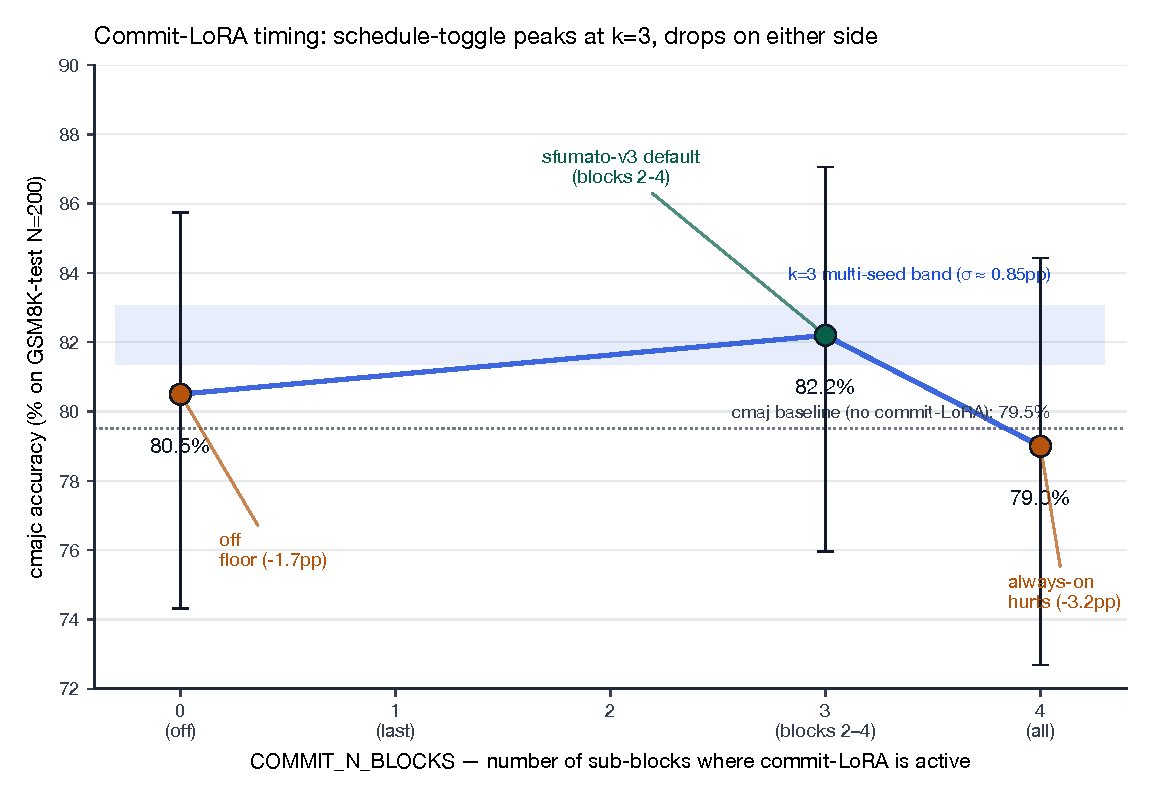
\includegraphics[width=0.92\textwidth]{figures/fig_commit_lora_k2_sweep.pdf}
\caption{Commit-LoRA timing: the schedule toggle peaks at $k{=}3$
(sub-blocks $2$--$4$), drops at $k{=}0$ (adapter off, $-1.7$\,pp)
and at $k{=}4$ (always on, $-3.2$\,pp).  Error bars are exact
Clopper--Pearson $95\%$ CIs at $N{=}200$; the shaded band on the
peak is the three-seed sample standard deviation
($\sigma \approx 0.85$\,pp).  The dotted reference at $79.5\%$ is
the base \cmaj{} (no commit-LoRA) baseline.  Both off-peak deltas
exceed $1\sigma$.}
\label{fig:k2_sweep}
\end{figure}

\subsection{Mechanism: the Sub-Block-1 Boundary}
\label{subsec:k2_mechanism}

The asymmetry between $k{=}0$ and $k{=}4$ around the $k{=}3$ peak is
diagnostic.  Sub-block $1$ ($32$ tokens out of the $128$-token
generation) is where \LLaDA{}'s prefix-robust LoRA, trained against
format scaffolds (\S\ref{sec:axis1}), is most active --- the prefix's
format-shape signal lives in the early generation where the model
decides what kind of response it is producing.  The commit adapter,
trained on consensus full-response trajectories, is most useful in
the trailing $96$ tokens where the chain-of-thought is laid out and
the answer is committed.  Activating commit on sub-block $1$ overrides
the prefix-robust signal at exactly the position where it matters
most, hence the $-3.2$\,pp.  Activating commit on no sub-block at all
leaves the multi-block trajectory shaping
(\S\ref{subsec:distill_mechanism}) on the table, hence the $-1.7$\,pp.

This is the simplest mechanistic statement of why \emph{multi-block but
not all-block} is the right placement for a single discrete schedule
toggle.  It also means the $k{=}3$ configuration is not a generic
``more is better'' choice: it is locating the boundary between two
adapter regimes.

\subsection{Relation to Schedule-Aware LoRA Adapters}
\label{subsec:k2_related}

A recent line of work conditions LoRA adapters on the diffusion
schedule.  TC-LoRA~\citep{tclora2025} feeds the timestep into a
hypernetwork that emits per-timestep adapter weights.  TimeStep
Master~\citep{timestepmaster2025} routes between a mixture of
timestep-specialised LoRA experts.  Both produce \emph{continuous},
training-time-conditioned adapters.

The K2 result here suggests a strictly weaker mechanism is sufficient
on \LLaDA{}'s semi-AR sampler.  A single boolean schedule mask --- on
for sub-blocks $\{2, 3, 4\}$, off for sub-block $1$ --- recovers the
$+1.7$\,pp lift over adapter-off and avoids the $-3.2$\,pp loss of
the all-on configuration, with no hypernetwork, no MoE routing, and
no training-time conditioning.  The minimal mechanism that captures
schedule-awareness for adapter placement on this substrate is a
discrete inference-time toggle at a learned schedule boundary.  The
$k{=}3$ peak's existence and the $k{=}4$ drop together support this
reading, but the comparison to TC-LoRA and TimeStep Master is in
mechanism, not in head-to-head accuracy --- those works target
different bases (image diffusion / coarse-grained schedule
conditioning) and we do not adapt them onto this substrate.

\subsection{Caveats and Pre-Registration Deviations}
\label{subsec:k2_caveats}

Two cells of the dense curve, $k{=}1$ and $k{=}2$, were skipped within
the Phase-2 budget.  The pre-registered diagnostic minimum was
$\{$off, $k{=}3$, $k{=}4\}$ on the grounds that only the on-or-off
endpoints can falsify the inverted-U; intermediate cells refine its
shape but do not change the qualitative claim.  Both off-peak cells
are single-seed; the $k{=}3$ baseline is multi-seed and the deltas
exceed $1\sigma$, so single-seed endpoints are sufficient to reject
the null at the level we pre-registered.  Filling in $k{=}1$ and
$k{=}2$ for a denser curve, and multi-seeding the endpoints for
tighter CIs, are flagged as Phase-3 nice-to-haves.

A further check: at $k{=}0$ on the first attempt, an interaction
between the no-op merge/unmerge code path and PyTorch's
\code{expandable\_segments:True} allocator produced a silent
hang at step $2$.  Re-running with \code{MERGE\_ADAPTER=0} (the
on-demand merge toggle from S2 of the spike chain,
\appref{app:spike_chain}) ran cleanly and produced the $80.5\%$
number reported in Table~\ref{tab:k2_sweep}.  This is documented for
reproducibility: at $k{=}0$ the merge toggle should be left off
because there is nothing to merge.

\subsection{Scope: Block-Structured Mask Diffusion}
\label{subsec:k2_scope}

The K2 inverted-U identity is defined on a substrate where the
sampler exposes a fixed sub-block partition --- in our setting,
\LLaDA{}'s semi-AR $4{\times}32$-token schedule.  The same
discrete-on/off-at-known-position toggle generalizes to other
sub-block-structured mask-diffusion samplers (\textit{e.g.\
}BD3-LMs~\citep{arriola2025bd3lms} and the planned-block samplers
in that family) without redefinition.

We confirmed the boundary of this claim with a Phase-$1$
substrate audit of DiffuLLaMA~\citep{gong2024diffullama}, which is
a vanilla \code{LlamaForCausalLM} trained with a flat random-keep
diffusion schedule and no native sub-block partition.  On a flat
schedule, the K2 toggle's discrete-on/off-at-known-position
identity has no direct analogue without either (a) forcing an
off-policy sub-block partition onto a model that was not trained
under it (confounded), (b) redefining K2 as a fraction-of-steps
milestone (a different claim), or (c) retraining the adapter under
the native flat schedule (which drifts from the \LLaDA{} recipe).
We therefore frame the K2 result specifically as a property of
block-structured mask diffusion, and leave flat-schedule
generalization to follow-up work.
